\section{Результаты}
\subsection{Решение двумерной задачи}

Для сравнения полученных результатов использовано эталонное решение из статьи \cite{2DBench}. 

\begin{table}[htp]
\center
  \begin{tabular}{lcccc}
\hline
	Re = 1000 
		& $\psi$   	& $\omega$ 	& x 		& y \\
\hline	
	Benchmark 	& 0.118942 	& 2.067213 	& 0.5300   	& 0.5650 \\
	Present		& 0.11523	& 2.06984	& 0.539		& 0.563 \\
\hline 
\hline
	Re = 5000 
		& $\psi$   	& $\omega$ 	& x 		& y \\
\hline	
	Benchmark 	& 0.122233 	& 1.940732 	& 0.5150   	& 0.5433 \\
	Present		& 0.1236	& 1.9387	& 0.514		& 0.550 \\
\hline 
  \end{tabular}
\caption{Значения максимума функции тока $\psi$, значение завихренности $\omega$ в той же точке и координаты этой точки для представленного 
метода (Present) и эталонного решения (Benchmark) \cite{2DBench}. При Re = 1000 и Re = 5000. Крышка движется слева направо.}
\label{comp}
\end{table}



\begin{figure}[htp]
\centering
\includegraphics[width = 1\linewidth]{resultImg/1000.pdf}
\caption{Изображены слева направо функция тока, завихренность и поле давления. Re=1000}
\label{Re1000}
\end{figure}

\begin{figure}[htp]
\centering
\includegraphics[width = 1\linewidth]{resultImg/5000.pdf}
\caption{Изображены слева направо функция тока, завихренность и поле давления. Re=5000}
\label{Re5000}
\end{figure}

На графиках \ref{Re1000},\ref{Re5000} изображена структура стационарного течения при Re=1000 и Re=5000. В правом и левом нижних углах существуют обратные вихри.  

\subsection{Решение линеаризованной системы} 
\if 0
При равенстве волнового числа нулю, трехмерная задача эквивалентна двумерной исходной задаче. В этом случае $\Re_{crit}(0)$~--- число Рейнольдса, при котором двумерная задача теряет устойчивость к двумерным возмущениям. При числах Рейнольдса, меньших критического, в двумерной каверне существует двумерное стационарное течение. В статье \cite{lin-stability} представленно значение 8045.  
\fi


Расчет проводился при значениях числа Рейнольдса от 100 до 5000, изменяющегося с шагом 50, и значениях волнового числа от 1 до 20, изменяющихся с шагом 1. Если решать задачу при каждом значении числа Рейнольдса и волнового числа, всего нужно провести 2000 испытвний. Для того чтобы уменьшить число испытаний, был использован следующий алгоритм. Для нахождения $Re_{crit}(\alpha)$ используется значение $\Re_{crit}(\alpha - \Delta\alpha)$. Вычисляется $d = d(\Re_{crit}(\alpha - \Delta\alpha), \alpha)$ если d > 0, вычисляем новое значение d при увеличенном на $\Delta \Re$ числе Ренольдса, если d < 0~--- уменьшаем Re на $\Delta \Re$. Итерации повторяются, пока не будет найдено новое критическое число Рейнольдса. 
Таким образом можно сократить число испытаний примерно до 60. 

Численное решение спектральной задачи требует большого объема памяти, и уже на сетках $50 \times 50$ памяти персонального компьютера недостаточно для расчета. Такой сетки достаточно лишь для чисел Рейнольдса меньших 150. Для других чисел Рейнольдса, когда решить спектральную задачу не представляется возможным, линеаризованная система уравнений \ref{lin3D_first}--\ref{lin3D_last} интегрируется по времени до установления коэффициента затухания к значению декремента. Также при Re < 150 результаты, полученные прямым численным интегрированием и из решения спектральной задачи, можно сравнить для проверки правильности програмной реализации и теоретических выкладок, что и было успешно сделано. 
В таблице \ref{Re_al} представленны результаты расчета в сравнении с результатами, полученными в \cite{lin-stability}. При $\alpha = 15$ значении $\Re_{crit}$ было вычислено более точно, как как в этой точке достигается минимум.

\begin{table}[htp]
 \begin{tabular}{cccccc}
\hline
\hline
  \multicolumn{3}{c}{Бифуркация Андронова--Хопфа} & \multicolumn{3}{c}{Стационарные бифуркации} \\
  $\alpha$&	$\Re_{crit}(\alpha)$ \cite{lin-stability}&  Пр.&	$\alpha$&	$\Re_{crit}(\alpha)$ \cite{lin-stability}&  Пр. \\
\hline
  1&	8047&		-&	12&	925&		950\\ 
  2&	8046.6&		-&	13&	837.69&		850\\
  3&	4772.68&	4800&	14&	799.3&		800\\
  4&	4769.25&	4800&	15&	786&		790\\
  5&	1967.9&		1950&	16&	786&		790\\
  6&	1032&		1050&	17&	795.74&		800\\
  7&	932.5&		950&	18&	811.92&		850\\
  8&	939&		950&	19&	832.58&		850\\
  9&	1029.8&		1050&	20&	856&		900\\
  10&	1132&		1150\\
  11&	1040&		1050\\
\hline
 \end{tabular}
 \caption{Зависимость критического числа Рейнольдса от волнового числа. Для сравнения приведено решение из \cite{lin-stability}. }
 \label{Re_al}
\end{table}

\begin{figure}
  \center
  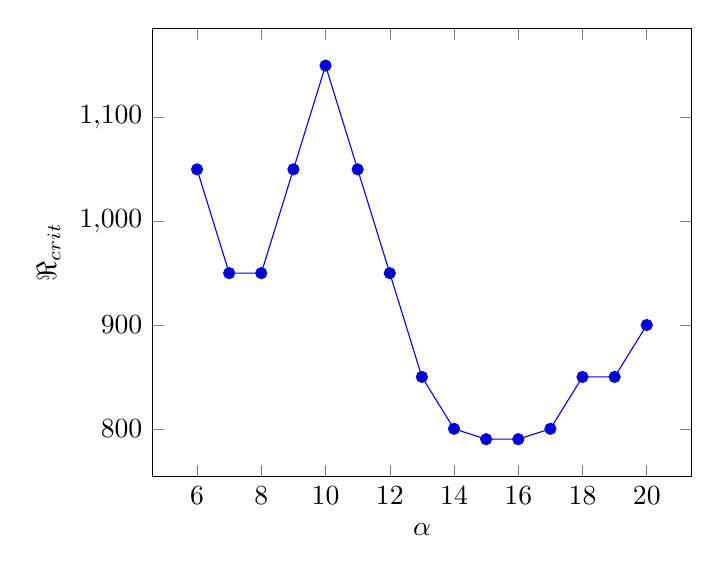
\begin{tikzpicture}
    \begin{axis}[
% 	xmode = log, ymode = log,
%	xmin = 0, ymin = 0,
	xlabel=$\alpha$,
	ylabel=$\Re_{crit}$ ]
      \addplot coordinates {
%	(3, 4800) (4, 4800) (5, 1950)
   (6, 1050) (7, 950) (8, 950) (9, 1050) (10, 1150)
	(11, 1050) (12, 950) (13, 850) (14, 800) (15, 790) (16, 790) (17, 800) (18, 850)
	(19, 850) (20, 900)};
    \end{axis}
  \end{tikzpicture}
  
  \caption{Кривая нейтральной стабильности}
  \label{graph:Re_al}
\end{figure}

Также кривая нейтральной стабильности изображена на графике \ref{graph:Re_al}. Кривая имеет два локальных минимума. Первый~--- при $\alpha \approx 7 $. В этой точке реализуется бифуркация Андронова--Хопфа. Второй~--- при $\alpha \approx 15$. В этой точке реализуется стационарная бифуркация. В таблице данные разделены на две колонки в соответствии с двумя механизмами возникновения неустойчивости.  Значения, достигаемые в первом и во втором локальных минимумах, сравнимы между собой, но при этом глобальный минимум достигается при $\alpha \approx 15$ и критическое число Рейнольдса в этой точке равно глобальному критическому числу Рейнольдся и составляет $\Re_{crit}^* = \Re_{crit}(15) = 790$. 

При расчете трехмерного течения нужны более плотные сетки по сравнению с расчетом двумерного течения \ref{2}. Под расчетом трехмерного течения понимается как прямой расчет линеаризованной системы уравнений \ref{3}, так и решение собственной задачи \ref{4}. На одной и той же сетке оба метода решают одну разностную задачу, и их решения должны совпадать. Если при Re=1000 для расчета \ref{2} достаточно $128 \times 128$, то для расчета \ref{3}--\ref{4} нужно от $196 \times 196$ узлов в сетке. Если для решения задачи \ref{2} на сетке $196 \times 196$ при том же Re=1000 шаг по времени был выбран 0.01, то для решения задачи \ref{3}--\ref{4} необходимо шаг уменьшить хотя бы до 0.002.  
